\chapter{Literature Review}

The rapid advancement of large language models (LLMs) has revolutionized natural language processing, demonstrating remarkable capabilities in tasks ranging from text generation to complex reasoning \cite{brown_2020_language, touvron_2023_llama}. However, the static nature of these models poses significant challenges when factual knowledge becomes outdated or requires correction. This chapter provides a comprehensive review of neural model editing techniques, with particular emphasis on the MEMIT and ROME algorithms that form the foundation of this research, alongside parameter-efficient fine-tuning methods such as LoRA and DoRA that offer complementary approaches to model adaptation.

\section{Foundations of Neural Model Editing}

\subsection{Knowledge Storage in Transformer Models}

Understanding how factual knowledge is stored and retrieved in transformer architectures is fundamental to developing effective editing techniques. Geva et al. \cite{geva_2021_transformer} provided seminal insights by proposing that transformer feed-forward layers function as key-value memories, where the first linear transformation acts as a key encoder and the second as a value retrieval mechanism. This conceptualization forms the theoretical foundation for direct weight editing approaches.

The transformer architecture, introduced by Vaswani et al. \cite{vaswani_2017_attention}, relies on multi-head attention mechanisms and position-wise feed-forward networks. Recent work has shown that factual associations are primarily stored in the middle layers of these networks, particularly within the multi-layer perceptron (MLP) components \cite{petroni_2019_language, jiang_2020_how}. This localization of factual knowledge storage has enabled targeted editing approaches that modify specific model weights without affecting the entire network.

\subsection{The Challenge of Catastrophic Forgetting}

Traditional fine-tuning approaches for updating model knowledge suffer from catastrophic forgetting, where learning new information interferes with previously acquired knowledge \cite{mccloskey_1989_catastrophic}. While techniques such as elastic weight consolidation have been proposed to mitigate this issue \cite{kirkpatrick_2017_overcoming}, they remain computationally expensive and may not be suitable for frequent knowledge updates. This limitation has motivated the development of more targeted editing approaches that can modify specific facts without extensive retraining.

% FIGURE PLACEHOLDER: Conceptual diagram showing knowledge storage in transformer layers and the catastrophic forgetting problem

\section{Direct Memory Editing Approaches}

\subsection{Early Knowledge Editing Methods}

The field of neural model editing emerged from early work on editable neural networks \cite{sinitsin_2020_editable_neural} and fact editing in language models \cite{cao_2021_editing_factual_knowledge}. These foundational approaches demonstrated the feasibility of modifying specific factual associations within pre-trained models, though they were limited in scale and often required significant computational resources.

Cao et al. \cite{cao_2021_editing_factual_knowledge} introduced one of the first systematic approaches to editing factual knowledge in language models, demonstrating that targeted modifications could be made to BERT-style models. However, their approach was limited to relatively simple factual updates and did not scale to large transformer models or multiple simultaneous edits.

\subsection{ROME: Rank-One Model Editing}

ROME (Rank-One Model Editing), introduced by Meng et al. \cite{meng_2022_locating}, represents a significant advancement in direct model editing techniques. The algorithm operates on the principle that factual associations can be modified through rank-one updates to specific feed-forward layers within transformer models.

\subsubsection{Rank-One Weight Updates}

ROME modifies the feed-forward weights using a rank-one update. For a target layer with weight matrix $\mathbf{W}$, the update takes the form:

\begin{equation}
\mathbf{W}_{new} = \mathbf{W}_{old} + \mathbf{u}\mathbf{v}^T
\end{equation}

where $\mathbf{u}$ and $\mathbf{v}$ are vectors chosen to ensure that the new association $(k^*, v^*)$ is correctly encoded while preserving existing associations. The optimization problem seeks to minimize:

\begin{equation}
\|\mathbf{W}_{new}\mathbf{K} - \mathbf{V}\|_F^2
\end{equation}

subject to the constraint that $\mathbf{W}_{new}\mathbf{k}^* = \mathbf{v}^*$, where $\mathbf{K}$ and $\mathbf{V}$ represent existing key-value associations.

\subsubsection{Evaluation and Limitations}

ROME demonstrates effectiveness on the zsRE (zero-shot Relation Extraction) benchmark, successfully editing individual facts while maintaining model performance on unrelated tasks. However, the algorithm faces several limitations:

\begin{itemize}
    \item \textbf{Sequential editing degradation}: Performance degrades significantly when applying multiple sequential edits
    \item \textbf{Scale limitations}: The rank-one constraint limits the complexity of edits that can be performed
    \item \textbf{Layer selection}: The method requires careful selection of target layers, which may vary across model architectures
\end{itemize}

\subsection{MEMIT: Mass-Editing Memory in a Transformer}

MEMIT (Mass-Editing Memory in a Transformer), developed by \cite{meng_2022_memit}, addresses the scalability limitations of ROME by enabling simultaneous editing of thousands of factual associations. This represents a significant advancement in neural model editing, scaling beyond previous methods by orders of magnitude.

\begin{figure}[H]
\centering
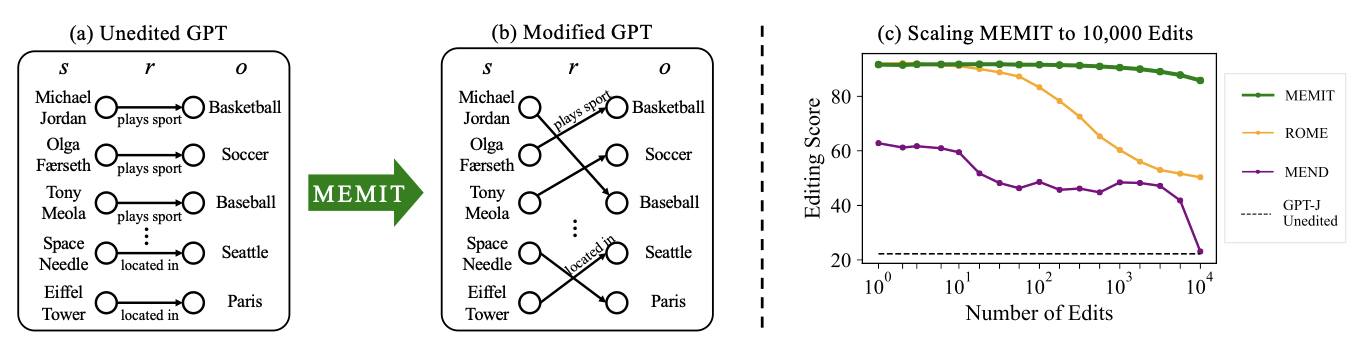
\includegraphics[width=0.85\textwidth]{figures/MEMIT_fig1.png}
\caption{MEMIT overview: (a) Language models store factual associations as (subject, relation, object) tuples, (b) MEMIT modifies these associations through targeted weight updates, and (c) performance comparison showing MEMIT's superior scaling capabilities, maintaining effectiveness up to 10,000 simultaneous edits compared to ROME and MEND methods.}
\label{fig:memit_overview}
\end{figure}

\subsubsection{Algorithmic Foundation}

Unlike ROME's single-fact editing approach, MEMIT formulates the editing problem as a batch optimization targeting multiple MLP layers simultaneously. The algorithm identifies critical layers where factual knowledge is stored and computes coordinated updates across these layers.

\begin{figure}[H]
\centering
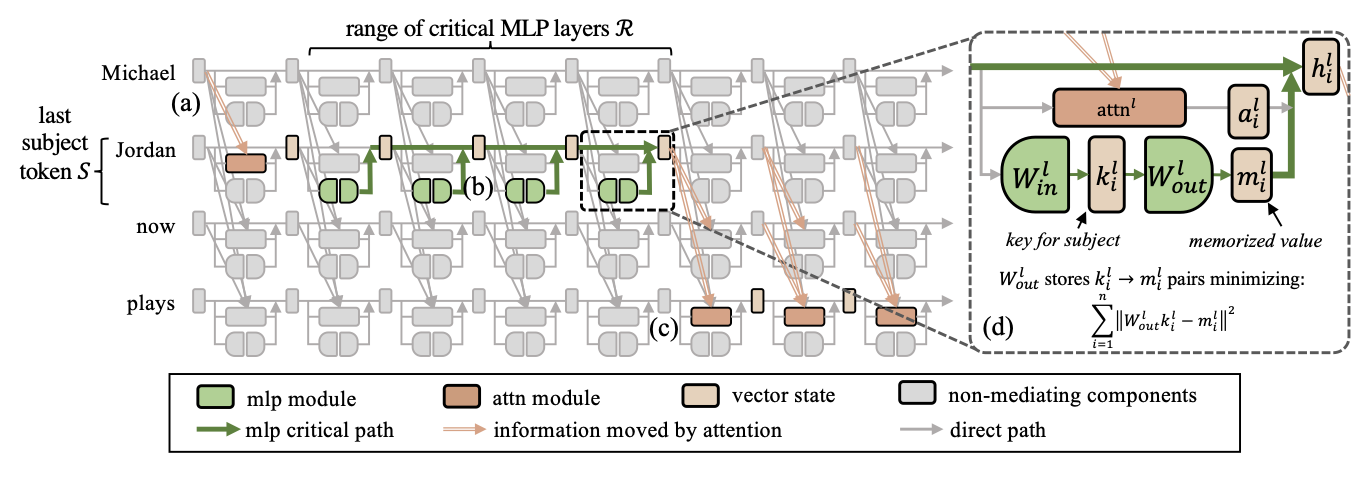
\includegraphics[width=0.95\textwidth]{figures/MEMIT_fig2.png}
\caption{MEMIT technical implementation showing the identification of critical MLP layers ($\mathcal{R}$) and the information flow during factual recall. The algorithm processes key-value pairs through multiple layers, with attention mechanisms (orange paths) and MLP modules (green paths) working together to store and retrieve factual associations.}
\label{fig:memit_technical}
\end{figure}

The multi-fact editing framework formulates the problem as a batch optimization:

\begin{equation}
\min_{\Delta\mathbf{W}} \|\mathbf{K}^T(\mathbf{W} + \Delta\mathbf{W}) - \mathbf{V}^T\|_F^2 + \lambda\|\Delta\mathbf{W}\|_F^2
\end{equation}

where $\mathbf{K}$ and $\mathbf{V}$ contain multiple key-value pairs to be edited simultaneously, and $\lambda$ controls the regularization strength to prevent overfitting.

\subsubsection{Covariance-Based Updates}

MEMIT employs a sophisticated approach based on estimating the covariance structure of the activations. The algorithm computes:

\begin{equation}
\mathbf{C} = \frac{1}{N}\sum_{i=1}^{N}\mathbf{k}_i\mathbf{k}_i^T
\end{equation}

where $\mathbf{k}_i$ represents the key vectors for the facts to be edited. This covariance matrix enables more stable updates when editing large numbers of facts simultaneously.

\subsubsection{Scaling and Performance}

MEMIT demonstrates remarkable scaling capabilities, successfully editing up to 10,000 facts simultaneously in GPT-J (6B parameters) and GPT-NeoX (20B parameters). The algorithm maintains three key properties:

\begin{enumerate}
    \item \textbf{Specificity}: Edits affect only the targeted facts without influencing unrelated knowledge
    \item \textbf{Generalization}: Edited facts generalize to paraphrases and related expressions
    \item \textbf{Fluency}: The model maintains natural language generation capabilities after editing
\end{enumerate}

Experimental results show that MEMIT achieves success rates exceeding 80\% on both the CounterFact and zsRE datasets when editing thousands of facts, significantly outperforming sequential application of ROME or other single-fact editing methods.

\section{Causal Tracing Methodology}

Causal tracing represents a fundamental technique for understanding information flow in transformer models and identifying the computational components responsible for specific behaviors. This methodology has become essential for both ROME and MEMIT algorithms in determining optimal target layers for knowledge editing.

\subsection{Theoretical Foundation}

The foundation of causal tracing lies in causal mediation analysis, which systematically identifies the causal role of intermediate representations in producing model outputs. The technique operates by:

\begin{enumerate}
    \item Running the model on a factual statement while introducing noise to disrupt normal processing
    \item Systematically restoring individual hidden states to identify which components are critical for fact retrieval
    \item Localizing the decisive computations to specific MLP modules in middle layers
\end{enumerate}

Mathematically, the causal effect of a hidden state $\mathbf{h}^{(l)}_i$ at layer $l$ and position $i$ is measured by comparing the model's output when this state is restored versus when it remains corrupted:

\begin{equation}
\mathcal{E}^{(l)}_i = \mathbb{E}[P(\text{fact} | \text{clean}_{<i}, \mathbf{h}^{(l)}_i, \text{corrupted}_{>i})] - \mathbb{E}[P(\text{fact} | \text{corrupted})]
\end{equation}

where $\mathcal{E}^{(l)}_i$ represents the causal effect of restoring the hidden state at layer $l$ and position $i$.

Both ROME and MEMIT leverage causal tracing to identify optimal target layers for knowledge editing. The technique reveals that factual knowledge is predominantly stored in middle layers of transformer models, with specific layer ranges varying across architectures. This localization enables targeted editing approaches that modify specific components while preserving overall model functionality.

% FIGURE PLACEHOLDER: Causal tracing visualization showing effect patterns across transformer layers

\section{Parameter-Efficient Fine-Tuning Methods}

While direct editing approaches like ROME and MEMIT offer precise control over factual associations, parameter-efficient fine-tuning (PEFT) methods provide complementary approaches for model adaptation. These techniques reduce the computational cost of fine-tuning while maintaining competitive performance.

\subsection{Adapter-Based Methods}

Early parameter-efficient approaches focused on introducing small adapter modules between transformer layers \cite{houlsby_2019_adapters}. These adapters contain significantly fewer parameters than full fine-tuning but can effectively adapt pre-trained models to downstream tasks. While not specifically designed for factual editing, adapters provide a foundation for understanding parameter-efficient model modification.

Prefix-tuning \cite{li_2021_prefix_tuning} and prompt-tuning \cite{lester_2021_prompt_tuning} represent alternative approaches that modify the input representation rather than the model weights. These methods demonstrate that effective adaptation can be achieved through careful manipulation of the input space, though they may be less suitable for precise factual editing tasks.

\subsection{LoRA: Low-Rank Adaptation}

LoRA (Low-Rank Adaptation), introduced by \cite{hu_2022_lora}, revolutionized parameter-efficient fine-tuning by decomposing weight updates into low-rank matrices. The core insight is that the weight changes during adaptation have low intrinsic rank.

\subsubsection{Mathematical Foundation}

For a pre-trained weight matrix $\mathbf{W}_0 \in \mathbb{R}^{d \times k}$, LoRA constrains the update $\Delta\mathbf{W}$ to be low-rank:

\begin{equation}
\mathbf{W} = \mathbf{W}_0 + \Delta\mathbf{W} = \mathbf{W}_0 + \mathbf{B}\mathbf{A}
\end{equation}

where $\mathbf{B} \in \mathbb{R}^{d \times r}$, $\mathbf{A} \in \mathbb{R}^{r \times k}$, and $r \ll \min(d,k)$ is the rank. During training, $\mathbf{W}_0$ is frozen and only $\mathbf{A}$ and $\mathbf{B}$ are updated.

\begin{figure}[H]
\centering
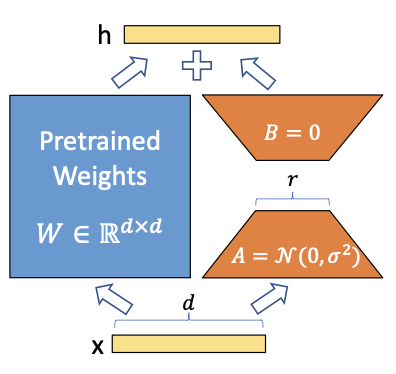
\includegraphics[width=0.5\textwidth]{figures/LoRA.png}
\caption{LoRA architecture showing the decomposition of weight updates into low-rank matrices. The original pre-trained weights $\mathbf{W}_0$ remain frozen while trainable low-rank matrices $\mathbf{A}$ and $\mathbf{B}$ capture the adaptation-specific changes.}
\label{fig:lora_architecture}
\end{figure}

\subsubsection{Efficiency and Performance}

LoRA achieves remarkable efficiency gains:
\begin{itemize}
    \item Reduces trainable parameters by up to 10,000$\times$ compared to full fine-tuning
    \item Decreases GPU memory requirements by 3$\times$
    \item Maintains or improves performance on downstream tasks
    \item Enables efficient switching between different task-specific adaptations
\end{itemize}

The method has been successfully applied to various transformer architectures, including GPT-3, where it achieves performance comparable to full fine-tuning while training only 0.01\% of the parameters.

\subsection{DoRA: Weight-Decomposed Low-Rank Adaptation}

DoRA (Weight-Decomposed Low-Rank Adaptation) \cite{liu_2024_dora} represents a recent advancement that addresses fundamental limitations in LoRA by decomposing weights into separate magnitude and direction components. This decomposition enables more nuanced parameter updates that better align with the patterns observed in full fine-tuning.

\subsubsection{Theoretical Foundation}

DoRA is motivated by empirical analysis showing that full fine-tuning and LoRA exhibit different patterns in terms of weight magnitude and direction changes. While LoRA only modifies the overall weight through additive low-rank updates, DoRA provides independent control over these two critical aspects of weight adaptation.

The method decomposes the pre-trained weight matrix as:

\begin{equation}
\mathbf{W}_0 = \mathbf{m} \frac{\mathbf{V}}{\|\mathbf{V}\|_c}
\end{equation}

where $\mathbf{m} = \|\mathbf{W}_0\|_c$ represents the magnitude component and $\frac{\mathbf{V}}{\|\mathbf{V}\|_c}$ represents the unit directional component. During adaptation, DoRA applies LoRA-style low-rank updates to the directional component while making the magnitude independently trainable:

\begin{equation}
\mathbf{W}' = \mathbf{m}' \frac{\mathbf{V} + \Delta\mathbf{V}}{\|\mathbf{V} + \Delta\mathbf{V}\|_c}
\end{equation}

where $\Delta\mathbf{V} = \mathbf{B}\mathbf{A}$ follows the standard LoRA decomposition and $\mathbf{m}'$ is the trainable magnitude parameter.

\begin{figure}[H]
\centering
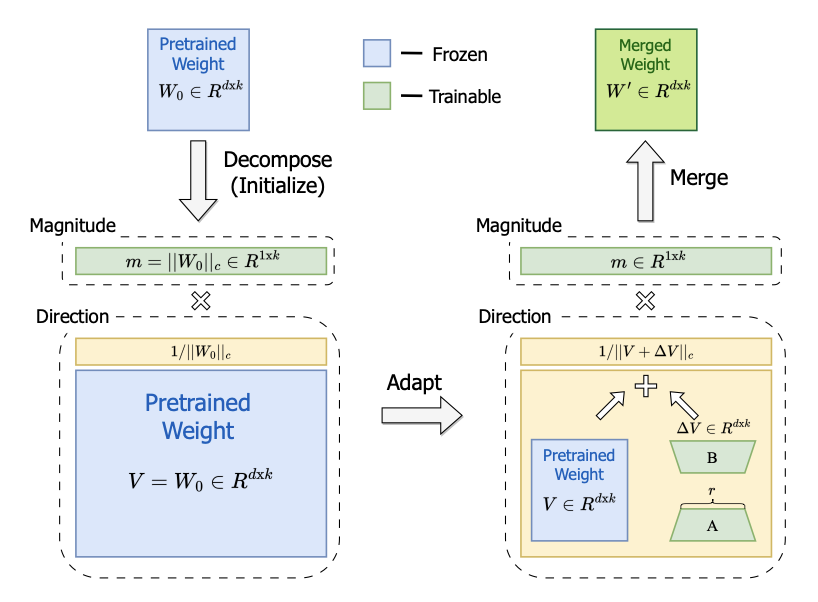
\includegraphics[width=0.7\textwidth]{figures/DoRA.png}
\caption{DoRA architecture showing the decomposition of pretrained weights into magnitude and direction components. The magnitude becomes independently trainable while the direction is updated using LoRA-style low-rank adaptation, providing more flexible parameter updates than standard LoRA.}
\label{fig:dora_architecture}
\end{figure}

\subsubsection{Advantages Over LoRA}

DoRA consistently outperforms LoRA across various tasks by addressing key limitations:

\begin{itemize}
    \item \textbf{Enhanced representational capacity}: Independent magnitude and direction control enables more flexible weight updates
    \item \textbf{Better fine-tuning alignment}: Weight update patterns more closely match those observed in full fine-tuning
    \item \textbf{Improved task performance}: Superior results on commonsense reasoning, visual instruction tuning, and multimodal understanding
    \item \textbf{Maintained efficiency}: Parameter count remains comparable to LoRA while providing enhanced learning capacity
\end{itemize}

The key insight is that magnitude and direction changes serve different roles in adaptation, and treating them independently allows for more effective parameter-efficient fine-tuning that bridges the gap between LoRA and full fine-tuning approaches.

\section{Evaluation Frameworks and Benchmarks}

\subsection{Knowledge Editing Benchmarks}

The evaluation of knowledge editing methods relies on established benchmarks that test different aspects of factual knowledge modification. Two primary datasets serve as the foundation for most knowledge editing research, each with distinct evaluation matrices and objectives.

\subsubsection{CounterFact Dataset}

The CounterFact dataset serves as a comprehensive benchmark for evaluating counterfactual knowledge editing. Each example consists of a factual statement and its counterfactual counterpart, enabling systematic evaluation of editing precision and generalization capabilities.

\textbf{Evaluation Matrix Structure:}
CounterFact employs a structured evaluation framework focusing on:
\begin{itemize}
    \item \textbf{Rewrite Success Rate}: Direct measurement of successful factual updates
    \item \textbf{Paraphrase Accuracy}: Generalization to rephrased versions of the target fact
    \item \textbf{Neighborhood Preservation}: Maintenance of related but unedited factual knowledge
    \item \textbf{Fluency Preservation}: Overall language generation quality post-editing
\end{itemize}

The dataset's strength lies in its controlled counterfactual structure, which allows for precise measurement of editing effects while minimizing confounding variables.

\subsubsection{zsRE: Zero-shot Relation Extraction}

The zsRE (Zero-shot Relation Extraction) benchmark \cite{petroni_2019_language} focuses on relational knowledge extraction and modification. Unlike CounterFact's counterfactual approach, zsRE tests the model's ability to extract and edit relational knowledge patterns without explicit training on the target relations.

\textbf{Evaluation Matrix Structure:}
zsRE employs a different evaluation framework emphasizing:
\begin{itemize}
    \item \textbf{Relation Extraction Accuracy}: Success in identifying and modifying relational patterns
    \item \textbf{Cross-relation Generalization}: Ability to generalize edits across similar relation types
    \item \textbf{Template Robustness}: Performance across different query templates and formats
    \item \textbf{Consistency Maintenance}: Preservation of logical consistency in related relations
\end{itemize}

The fundamental difference between zsRE and CounterFact lies in zsRE's focus on relational structures rather than individual factual statements, requiring more sophisticated handling of knowledge interdependencies.


\subsection{Evaluation Metrics}

Knowledge editing evaluation typically focuses on three key criteria:

\begin{enumerate}
    \item \textbf{Rewrite Success}: Whether the model correctly produces the new factual association
    \item \textbf{Paraphrase Generalization}: Whether the edit generalizes to paraphrases of the original fact
    \item \textbf{Neighborhood Preservation}: Whether related but unedited facts remain unchanged
\end{enumerate}

Additional metrics include fluency preservation, measured through perplexity on held-out text, and downstream task performance to ensure that editing does not degrade general capabilities.

\subsection{Ripple Effects and Unintended Consequences}

Recent research has highlighted the importance of evaluating ripple effects of knowledge editing \cite{wang_2023_ripple_effects}. When a fact is edited, it may have unintended consequences on related facts or reasoning chains. For example, changing "The president of the USA is Biden" might affect other facts about American politics or government structure.

The evaluation of ripple effects requires careful consideration of:
\begin{itemize}
    \item Semantic similarity between edited and potentially affected facts
    \item Logical consistency in multi-fact scenarios
    \item Long-term stability of edits over multiple inference steps
\end{itemize}

% FIGURE PLACEHOLDER: Evaluation framework diagram showing the three main criteria and their relationships

\section{Challenges and Limitations}

\subsection{Scalability Constraints}

Despite advances in methods like MEMIT, scalability remains a significant challenge:
\begin{itemize}
    \item Memory requirements grow quadratically with the number of edits
    \item Computational complexity increases substantially for large-scale editing
    \item Model-specific layer selection requires manual tuning
\end{itemize}

\subsection{Cross-Model Generalization}

Most editing methods are developed and evaluated on specific model architectures. Transfer to different architectures (e.g., from GPT to LLaMA) often requires significant adaptation, limiting the generalizability of existing approaches.

\subsection{Evaluation Gaps}

Current evaluation frameworks have several limitations:
\begin{itemize}
    \item Limited coverage of complex reasoning scenarios
    \item Insufficient evaluation of long-term stability
    \item Lack of standardized protocols for ripple effect assessment
\end{itemize}

\subsection{Integration Challenges}

The relationship between direct editing methods and parameter-efficient fine-tuning remains underexplored. Developing unified frameworks that leverage both approaches presents significant technical challenges in terms of optimization dynamics and knowledge preservation.

\section{Summary and Research Gaps}

This literature review has examined the current state of neural model editing, with particular focus on MEMIT and ROME algorithms, alongside parameter-efficient fine-tuning methods such as LoRA and DoRA. The field has made significant progress in developing methods for targeted fact editing and efficient model adaptation.

Key achievements include:
\begin{itemize}
    \item Development of scalable editing methods (MEMIT) capable of handling thousands of simultaneous edits
    \item Precise localization techniques (causal tracing) for identifying critical model components
    \item Highly efficient adaptation methods (LoRA, DoRA) that maintain performance while drastically reducing computational requirements
    \item Comprehensive evaluation frameworks for assessing editing quality and side effects
\end{itemize}

However, several research gaps remain:

\subsubsection{Layer Selection Optimization}
Current methods rely on heuristic or model-specific approaches for selecting target layers. A systematic methodology for optimal layer selection across different architectures represents a significant opportunity for improvement.

\subsubsection{Multi-Scale Editing Analysis}
While MEMIT demonstrates large-scale editing capabilities, comprehensive analysis of editing effectiveness across different scales (from single facts to tens of thousands) remains limited. Understanding the scaling behavior is crucial for practical applications.

\subsubsection{Integration of Editing and Fine-tuning}
The relationship between direct editing methods and parameter-efficient fine-tuning is underexplored. Developing unified frameworks that leverage both approaches could provide significant advantages.

\subsubsection{Cross-Architecture Generalization}
Most existing work focuses on specific model families. Developing editing methods that generalize across different transformer architectures (e.g., decoder-only vs. encoder-decoder models) remains an open challenge.

\subsubsection{Unexplored Model Architectures}
A critical gap exists in the exploration of neural model editing on recently developed architectures. The LLaMA model family, particularly \textbf{meta-llama/Llama-3.1-8B-Instruct}, represents a significant advancement in open-source language modeling. This model builds upon the foundational LLaMA architecture with substantial improvements in instruction following capabilities and multilingual performance \cite{dubey_2024_llama3}. The model employs a decoder-only transformer architecture with optimized attention mechanisms and has been fine-tuned specifically for instruction-following tasks, making it an ideal candidate for knowledge editing research due to its factual knowledge retention and generalization capabilities.

Similarly, \textbf{DeepSeek-R1-Distill-Llama-8B represents an entirely novel target for knowledge editing research—no prior work has investigated editing capabilities on this architecture}. This distilled model combines the architectural benefits of the LLaMA foundation with specialized knowledge distillation techniques, potentially offering different knowledge storage patterns that could affect editing effectiveness. The comparative study of these two architectures provides unprecedented insights into how different training methodologies and architectural optimizations influence knowledge editing performance.

This dissertation addresses several of these gaps by developing novel layer selection methodologies based on causal tracing analysis, conducting comprehensive multi-scale evaluation across different model architectures, and investigating the integration of editing techniques with parameter-efficient fine-tuning approaches. \textbf{Crucially, this work presents the first comprehensive study of neural model editing on DeepSeek-R1-Distill-Llama-8B, establishing foundational knowledge for editing this advanced architecture.} The following chapters detail the methodology and experimental results that advance the state of knowledge in neural model editing.